% =============================================================
% Capitulo 5 - Seleccion del microcontrolador y arquitectura general
% =============================================================

\chapter{Selección del microcontrolador y arquitectura general de periféricos}
\label{cap:micro}
\section{Requisitos de diseño}

Como base para el software de control, se partió del programa previamente desarrollado por el NIES, descrito en el Anexo \ref{anexo:hsrlnies}. Este software, pese a tener problemas de estabilidad y de compatibilidad con los sistemas operativos actuales, sirvió como referencia para definir la potencia de cómputo necesaria que debería tener el microcontrolador a seleccionar. 

Además, se tomaron los siguientes requisitos de periféricos para el microcontrolador a usar:

\begin{itemize}
    \item \textbf{Comunicación con PC:} realizada mediante un puerto USB.
    \item \textbf{Comunicación con seeder:} mediante puerto serie, usando RS-232.
    \item \textbf{Digitalización de señal del detector de picos:} utilizando un ADC. Idealmente el mismo del microcontrolador para reducir cantidad de componentes y costo.
    \item \textbf{Detección de flanco de sincronía del láser}: con GPIO de uso general.
\end{itemize}

\section{Microcontroladores de la familia RP2350}
\label{sec:rp2350}

Se seleccionó un RP2350 (presente en la placa de desarrollo Raspberry Pi Pico~2) como microcontrolador del sistema debido a su bajo costo y a su documentación técnica completa y accesible. Además, al contar con dos interfaces UART, USB nativo y 26 pines GPIO, no sólo permite la comunicación con el \emph{seeder} y la PC, sino que además habilita la expansión del sistema en caso de ser necesario. Para el prototipo de la placa de control se utilizó el módulo comercial Raspberry Pi Pico 2 como referencia de diseño.

Sus dos núcleos permiten correr en paralelo lecturas y escrituras de puerto serie y la digitalización de la señal, sin necesidad de utilizar sistemas de división de tareas o interrupciones específicas mediante timers. Las características más importantes del microcontrolador se resumen en la Tabla \ref{tab:rp2350} \cite{rp2350_datasheet}. El agregado de protocolo I2C también permite ampliar al sistema con un diverso rango de sensores compatibles con este protocolo. El diagrama de pinouts del mismo se representa en la Figura \ref{fig:pinout}.

\begin{figure}
    \centering
    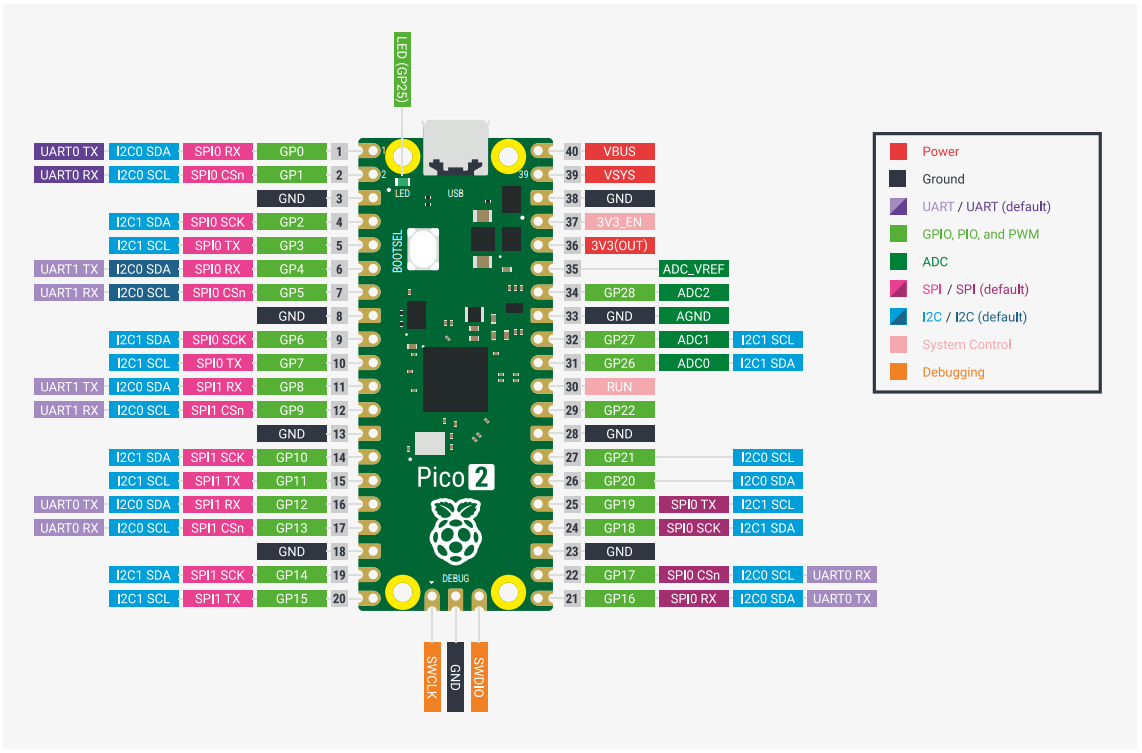
\includegraphics[width=0.8\textwidth]{figuras/5_pinout.png}
    \caption{Pinout de la placa de desarrollo Raspberry Pi Pico 2 (Fuente: adaptado de \cite{rp2350_datasheet}).}
    \label{fig:pinout}
\end{figure}

\begin{table}[h]
\centering
\renewcommand{\arraystretch}{1.3}
\begin{tabularx}{0.9\textwidth}{>{\bfseries}l X}
\toprule
Característica & \textbf{Especificación (Microcontrolador RP2350)} \\
\midrule
Arquitectura & Doble núcleo ARM Cortex-M33 / Doble núcleo Hazard3 RISC-V \\
Frecuencia de reloj & 150 MHz \\
Memoria SRAM & 520 KB integrada \\
Pines GPIO (RP2350A) & 30 en total (26 expuestos en la placa Pico 2) \\
Periféricos estándar & 2 $\times$ UART, 2 $\times$ SPI, 2 $\times$ I2C \\
Canales PWM & 24 canales \\
Convertidor A/D (ADC) & 4 canales de 12 bits \\
E/S Programable (PIO) & 3 bloques PIO (12 máquinas de estado en total) \\
Seguridad & ARM TrustZone, Secure Boot, SRAM con Anti-tamper, 8 KB OTP \\
\bottomrule
\end{tabularx}
\vspace{0.2cm}
\caption{Especificaciones destacadas del RP2350, utilizado en la Raspberry Pi Pico 2 (Fuente: adaptado de \cite{rp2350_datasheet}).}
\label{tab:rp2350}
\end{table}

Durante la selección del microcontrolador se evaluaron otras alternativas disponibles comercialmente, tales como el STM32F103C8T6 o el ESP32-WROOM-32. Como se resume en la Tabla \ref{tab:comparacion_micro}, ninguna de las tres opciones presenta limitaciones de cómputo frente a los requisitos planteados, por lo que la decisión se apoyó en
criterios de periféricos, documentación, costo, disponibilidad y familiaridad previa.
El ESP32-WROOM-32 fue descartado por carecer de interfaz USB nativa (obligando a incorporar un puente USB-serie adicional en la placa). El STM32F103C8T6, si bien es la opción de menor costo y con mejor ADC, posee documentación más diluida lo que podría aumentar los tiempos de desarrollo.

\begin{table}[h]
\centering
\renewcommand{\arraystretch}{1.3}
\begin{tabularx}{\textwidth}{>{\bfseries}l X X X}
\toprule
Criterio & \textbf{RP2350 (Pico 2)} & \textbf{STM32F103C8T6} & \textbf{ESP32-WROOM-32} \\
\midrule
Núcleos / frecuencia & 2 $\times$ Cortex-M33 @ 150 MHz & 1 $\times$ Cortex-M3 @ 72 MHz & 2 $\times$ Xtensa LX6 @ 240 MHz \\
SRAM & 520 KB & 20 KB & 520 KB \\
Memoria de programa & 4 MB QSPI externa & 64 KB Flash & 4 MB QSPI externa \\
ADC integrado & SAR 12 bits, 4 canales, 500 kS/s & SAR 12 bits, 10 canales, 1 MS/s & SAR 12 bits, 18 canales, con no linealidad y ruido documentados \\
UART & 2 & 3 & 3 \\
USB nativo & USB 1.1 device/host & USB 2.0 FS (solo device) & No posee; requiere puente USB-serie externo \\
GPIO expuestos & 26 & 32 & 34 (varios de solo entrada) \\
Documentación & Datasheet unificado y SDK en C con ejemplos oficiales & Reference manual extenso, aprendizaje pronunciado & Documentación repartida entre ESP-IDF y datasheet \\
Costo aproximado (placa) & USD 5--7 & USD 3--5 & USD 5--7 \\
Disponibilidad en distribuidores locales & Alta & Alta, aunque predominan clones no oficiales & Alta \\
Familiaridad previa & Sí & No & Parcial \\
\bottomrule
\end{tabularx}
\vspace{0.2cm}
\caption{Comparación de las alternativas de microcontrolador evaluadas (Fuente: elaboración propia a partir de \cite{rp2350_datasheet, stm32f103_datasheet, esp32_datasheet}).}
\label{tab:comparacion_micro}
\end{table}

\section{Selección del conversor analógico digital}

El microcontrolador RP2350 cuenta con un conversor analógico de cuatro canales de muestreo. Si bien durante el desarrollo del presente trabajo se trabajó únicamente con los canales $P_+$ y $P_-$, la lectura de los dos haces centrales $P_0$ puede constituir un dato de interés para el control del sistema. La disponibilidad de canales analógicos adicionales deja abierta esa posibilidad sin necesidad de modificar el hardware.

El microcontrolador RP2350 incorpora un convertidor analógico-digital de aproximaciones sucesivas (SAR) de 12 bits, cuya frecuencia de reloj de conversión \texttt{clk\_adc} opera nominalmente a $48\,\mathrm{MHz}$. Cada conversión completa (incluyendo la etapa de muestreo y retención y la posterior aproximación sucesiva) demanda 96 ciclos de dicho reloj, de donde se obtiene el tiempo de conversión mínimo:

\begin{equation}
    t_{\mathrm{conv}} = \frac{96\ \mathrm{ciclos}}{48 \times 10^{6}\,\mathrm{Hz}} = 2\,\mu\mathrm{s}
    \label{eq:tconv_rp2350}
\end{equation}

Este valor establece una frecuencia máxima de muestreo de $500\,\mathrm{kS/s}$. Tiempo suficiente para realizar el muestreo de la señal obtenida del detector de picos. La configuración del ADC en software, para máxima velocidad de conversión se encuentra detallada en la Tabla \ref{tab:config_adc}.


\begin{table}[h]
\centering
\begin{tabular}{lll}
\hline
\textbf{Parámetro} & \textbf{Valor} & \textbf{Constante} \\
\hline
Resolución & 12 bits & --- \\
Reloj del ADC & $48\,\mathrm{MHz}$ & --- \\
Divisor de reloj & 0 (máxima velocidad) & \texttt{ADC\_CLOCK\_DIV} \\
Ciclos por conversión & 96 & --- \\
Tiempo de conversión & $2\,\mu\mathrm{s}$ & --- \\
Frecuencia de muestreo total & $500\,\mathrm{kS/s}$ & --- \\
Canales activos & 2 (round-robin) & \texttt{ADC\_CHAN\_0/1} \\
Entradas analógicas & GPIO26, GPIO27 & \texttt{ADC\_GPIO\_0/1} \\
Frecuencia por canal & $250\,\mathrm{kS/s}$ & --- \\
Muestras por captura & 1024 (512 por canal) & \texttt{NUM\_SAMPLES} \\
Duración de la captura & $2{,}048\,\mathrm{ms}$ & --- \\
Disparo & Flanco ascendente, GPIO2 & \texttt{TRIGGER\_PIN} \\
Transferencia & DMA sincronizado por \texttt{DREQ\_ADC} & --- \\
\hline
\end{tabular}
\caption{Configuración del ADC del RP2350 en el sistema de adquisición (Fuente: elaboración propia).}
\label{tab:config_adc}
\end{table}


\section{Comunicación serie RS-232/UART}
\label{sec:rs232_uart}

La comunicación entre la placa de control y el láser \emph{seeder} se realiza mediante puerto serie estándar RS-232 especificado por el fabricante del equipo \cite{npphotonics_flm005}. Dado que los niveles de tensión RS-232
no son compatibles con los niveles de tensión lógicos del microcontrolador, es necesario un circuito integrado transceptor que adapte ambos.

\begin{figure}[htpb]
    \centering
    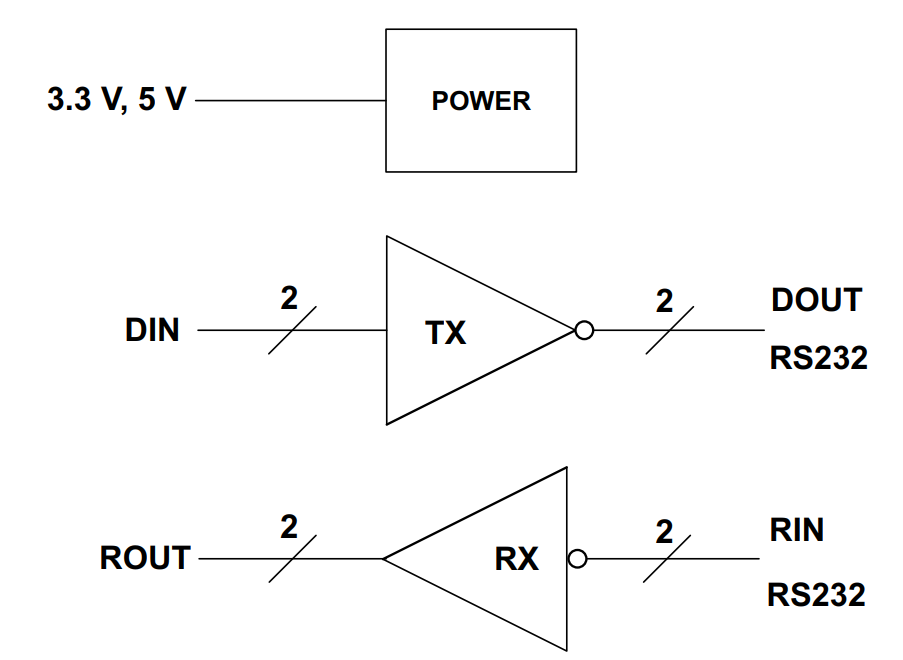
\includegraphics[width=0.6\textwidth]{figuras/5_max3232.png}
    \caption{Esquemático simplificado del transceptor MAX3232 (Fuente: adaptado de \cite{ti_max3232}).}
    \label{fig:max3232}
\end{figure}

Para la tarea de adaptar niveles de tensión se seleccionó el circuito integrado MAX3232 por su simplicidad de implementación, alta disponibilidad y baja cantidad de componentes requeridos. Además, gracias a la posibilidad de alimentarlo con 3,3~V \cite{ti_max3232}, es posible utilizar la salida del regulador de la misma placa de desarrollo Raspberry Pi Pico 2. Su diagrama simplificado se representa en la Figura \ref{fig:max3232}.


\section{Detección de la señal de sincronismo}

El láser \emph{host} provee una señal de sincronismo SYNC para detectar cuándo ocurre el disparo del mismo. Para la correcta digitalización, es necesario comenzar la conversión en el momento que el láser dispara para digitalizar el valor del detector de picos antes de que el mismo se descargue por completo.

Esta señal se adaptó de niveles TTL a niveles CMOS mediante el uso de un simple divisor resistivo, ilustrado en la Figura \ref{fig:divisor}.

Para la selección de resistencias

\begin{equation}
  3{,}3\,\text{V} = 5\,\text{V} \, \frac{R_{18}}{R_{17} + R_{18}}   
  \label{eq:div1}
\end{equation}

\noindent con $R_{17} = 1{,}8\,\text{k}\Omega$, se tiene

\begin{equation}
  R_{18} = \frac{1188}{0{,}34} \approx 3494{,}12\,\Omega \approx 3{,}494\,\text{k}\Omega  
  \label{eq:div2}
\end{equation}

\noindent por lo tanto según valores estándar E24 $R_{18} = 3{,}6\,\text{k}\Omega$

\begin{figure}[h]
    \centering
    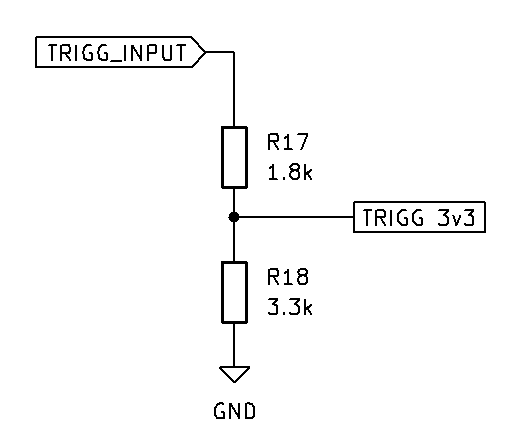
\includegraphics[width=0.5\textwidth]{figuras/5_divisor.png}
    \caption{Divisor resistivo para la señal de sincronismo del láser host (Fuente: elaboración propia).}
    \label{fig:divisor}
\end{figure}